\documentclass[journal]{IEEEtran}
\usepackage[a5paper, margin=10mm]{geometry}
%\usepackage{lmodern} % Ensure lmodern is loaded for pdflatex
\usepackage{tfrupee} % Include tfrupee package


\setlength{\headheight}{1cm} % Set the height of the header box
\setlength{\headsep}{0mm}     % Set the distance between the header box and the top of the text


%\usepackage[a5paper, top=10mm, bottom=10mm, left=10mm, right=10mm]{geometry}

%
\setlength{\intextsep}{10pt} % Space between text and floats

\makeindex


\usepackage{cite}
\usepackage{amsmath,amssymb,amsfonts,amsthm}
\usepackage{algorithmic}
\usepackage{graphicx}
\usepackage{textcomp}
\usepackage{xcolor}
\usepackage{txfonts}
\usepackage{listings}
\usepackage{enumitem}
\usepackage{mathtools}
\usepackage{gensymb}
\usepackage{comment}
\usepackage[breaklinks=true]{hyperref}
\usepackage{tkz-euclide} 
\usepackage{listings}
\usepackage{multicol}
\usepackage{xparse}
\usepackage{gvv}
%\def\inputGnumericTable{}                                 
\usepackage[latin1]{inputenc}                  
\usepackage{color}                                            
\usepackage{array}                                          
\usepackage{longtable}                                       
\usepackage{calc}                                             
\usepackage{multirow}                                         
\usepackage{hhline}                                           
\usepackage{ifthen}                                           
\usepackage{lscape}
\usepackage{tabularx}
\usepackage{array}
\usepackage{float}
\usepackage{ar}
\usepackage[version=4]{mhchem}


\newtheorem{theorem}{Theorem}[section]
\newtheorem{problem}{Problem}
\newtheorem{proposition}{Proposition}[section]
\newtheorem{lemma}{Lemma}[section]
\newtheorem{corollary}[theorem]{Corollary}
\newtheorem{example}{Example}[section]
\newtheorem{definition}[problem]{Definition}
\newcommand{\BEQA}{\begin{eqnarray}}
\newcommand{\EEQA}{\end{eqnarray}}

\theoremstyle{remark}


\begin{document}
\bibliographystyle{IEEEtran}
\onecolumn

\title{METALLURGY ENGINEERING}
\author{GATE 2021\\
EE25BTECH11027-INDHIRESH S
}
\maketitle


\renewcommand{\thefigure}{\theenumi}
\renewcommand{\thetable}{\theenumi}

\section*{General Aptitude}
\subsection*{Q1 - Q5 carry one mark each  (for each wrong answer: - 1/3)}
\begin{enumerate}
\item Five persons P, Q, R, S and T are to be seated in a row, all facing the same direction, but not necessarily in the same order. P and T cannot be seated at either end of the row. P should not be seated adjacent to S. R is to be seated at the second position from the left end of the row. The number of distinct seating arrangements possible is: \hfill{\brak{\text{GATE MT 2021}}}
\begin{multicols}{4}
\begin{enumerate}
\item $2$
\item $3$
\item $4$
\item $5$
\end{enumerate}
\end{multicols}

\item Consider the following sentences: \hfill{\brak{\text{GATE MT 2021}}} 
\begin{enumerate}[label=\Alph*), start=16]
  \item  The number of candidates who appear for the GATE examination is staggering.
  \item  A number of candidates from my class are appearing for the GATE examination.
  \item  The number of candidates who appear for the GATE examination are staggering.
  \item  A number of candidates from my class is appearing for the GATE examination.
\end{enumerate}
Which of the above sentences are grammatically CORRECT?
\begin{multicols}{4}
\begin{enumerate}
\item (P) and (Q)
\item (P) and (R)
\item (Q) and (R)
\item (R) and (S)
\end{enumerate}
\end{multicols}

\item A digital watch X beeps every 30 seconds while watch Y beeps every 32 seconds. They beeped together at 10 AM. The immediate next time that they will beep together is \hfill{\brak{\text{GATE MT 2021}}}
\begin{multicols}{4}
\begin{enumerate}
\item 10.08 AM
\item 10.42 AM
\item 11.00 AM
\item 10.00 PM
\end{enumerate}
\end{multicols}

\item If $\oplus\div\odot=2$; $\oplus\div4=3$; $2\times\oplus=6$; $\Delta\times\otimes=10$. Then, the value of $(\otimes-\oplus)^{2}$, is: \hfill{\brak{\text{GATE MT 2021}}}
\begin{multicols}{4}
\begin{enumerate}
\item 0
\item 1
\item 4
\item 16
\end{enumerate}
\end{multicols}

\item The front door of Mr. X's house faces East. Mr. X leaves the house, walking 50 m straight from the back door that is situated directly opposite to the front door. He then turns to his right, walks for another 50 m and stops. The direction of the point Mr. X is now located at with respect to the starting point is \hfill{\brak{\text{GATE MT 2021}}}
\begin{multicols}{4}
\begin{enumerate}
\item South-East
\item North-East
\item West
\item North-West
\end{enumerate}
\end{multicols}

\subsection*{Q6 - Q10 carry two marks each (for each wrong answer: - 2/3).}

\item Given below are two statements 1 and 2, and two conclusions I and II. \hfill{\brak{\text{GATE MT 2021}}}\\
Statement 1: All entrepreneurs are wealthy. \\
Statement 2: All wealthy are risk seekers. \\
Conclusion I: All risk seekers are wealthy. \\
Conclusion II: Only some entrepreneurs are risk seekers. \\
Based on the above statements and conclusions, which one of the following options is CORRECT?
\begin{enumerate}
\item Only conclusion I is correct
\item Only conclusion II is correct
\item Neither conclusion I nor II is correct
\item Both conclusions I and II are correct
\end{enumerate}

\item A box contains 15 blue balls and 45 black balls. If 2 balls are selected randomly, without replacement, the probability of an outcome in which the first selected is a blue ball and the second selected is a black ball, is \hfill{\brak{\text{GATE MT 2021}}}
\begin{multicols}{4}
\begin{enumerate}
\item $\frac{3}{16}$
\item $\frac{45}{236}$
\item $\frac{1}{4}$
\item $\frac{3}{4}$
\end{enumerate}
\end{multicols}

\item The ratio of the area of the inscribed circle to the area of the circumscribed circle of an equilateral triangle is \hfill{\brak{\text{GATE MT 2021}}}
\begin{figure}[H]
    \centering
    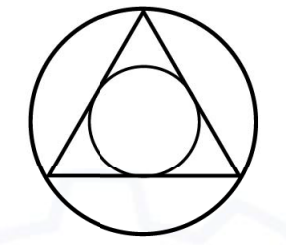
\includegraphics[width=0.2\columnwidth]{figs/Q.8 GA.png}
    \caption\centering{CIRCLE}
    \label{fig:placeholder}
\end{figure}
\begin{multicols}{4}
\begin{enumerate}
\item $\frac{1}{8}$
\item $\frac{1}{6}$
\item $\frac{1}{4}$
\item $\frac{1}{2}$
\end{enumerate}
\end{multicols}

\item Consider a square sheet of side 1 unit. The sheet is first folded along the main diagonal. This is followed by a fold along its line of symmetry. The resulting folded shape is again folded along its line of symmetry. The area of each face of the final folded shape, in square units, equal to \hfill{\brak{\text{GATE MT 2021}}}
\begin{multicols}{4}
\begin{enumerate}
\item $\frac{1}{4}$
\item $\frac{1}{8}$
\item $\frac{1}{16}$
\item $\frac{1}{32}$
\end{enumerate}
\end{multicols}

\item The world is going through the worst pandemic in the past hundred years. The air travel industry is facing a crisis, as the resulting quarantine requirement for travelers led to weak demand. In relation to the first sentence above, what does the second sentence do? \hfill{\brak{\text{GATE MT 2021}}}
\begin{enumerate}
\item Restates an idea from the first sentence.
\item Second sentence entirely contradicts the first sentence.
\item The two statements are unrelated.
\item States an effect of the first sentence.
\end{enumerate}
\end{enumerate}

\section*{Metallurgical Engineering}
\subsection*{Q1 - Q13 carry one mark each}
\begin{enumerate}
\item For the matrix given below, the eigenvalues are: \hfill{\brak{\text{GATE MT 2021}}}
\begin{align}
    \myvec{ 1 & 0 & -1 \\ 0 & 1 & 0 \\ -1 & 0 & 1} 
\end{align}
\begin{multicols}{4}
\begin{enumerate}
\item 0, 2, 2
\item 1, 1, 2
\item 0, 1, 2
\item 0, 1, 3
\end{enumerate}
\end{multicols}

\item Which one of the following is a homogeneous function of degree three? \hfill{\brak{\text{GATE MT 2021}}}
\begin{multicols}{2}
\begin{enumerate}
\item $x^{3}+2x^{2}y^{2}$
\item $y^{2}x+2yx^{2}$
\item $y^{3}+2x^{2}$
\item $xy^{2}+3xy$
\end{enumerate}
\end{multicols}

\item The divergence of a vector field $\vec{V}(x,y,z)$, where its three components $(V_{x}, V_{y}, V_{z})$ are functions of $x, y, z,$ is: \hfill{\brak{\text{GATE MT 2021}}}
\begin{multicols}{2}
    

\begin{enumerate}
\item $\frac{\partial V_{x}}{\partial x}+\frac{\partial V_{y}}{\partial y}+\frac{\partial V_{z}}{\partial z}$
\item $(\frac{\partial V_{z}}{\partial y}-\frac{\partial V_{y}}{\partial z})i+(\frac{\partial V_{x}}{\partial z}-\frac{\partial V_{z}}{\partial x})j+(\frac{\partial V_{y}}{\partial x}-\frac{\partial V_{x}}{\partial y})k$
\item $\frac{\partial V_{x}}{\partial x}i+\frac{\partial V_{y}}{\partial y}j+\frac{\partial V_{z}}{\partial z}k$
\item $\frac{\partial^{2}V_{x}}{\partial x^{2}}+\frac{\partial^{2}V_{y}}{\partial y^{2}}+\frac{\partial^{2}V_{z}}{\partial z^{2}}$
\end{enumerate}
\end{multicols}
\item Which one of the following is 'center split' defect in rolling operation? \hfill{\brak{\text{GATE MT 2021}}}
\begin{figure}[H]
    \centering
    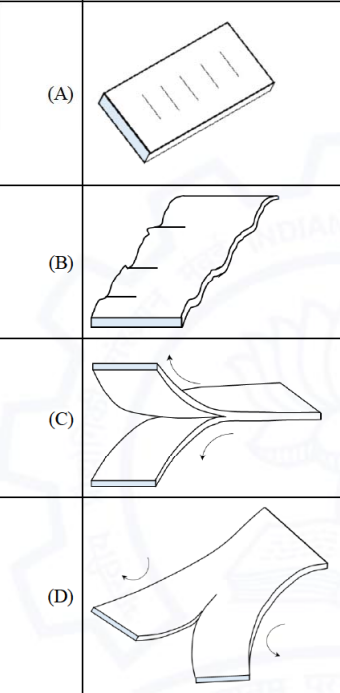
\includegraphics[width=0.3\columnwidth]{figs/Q.4.png}
    \caption\centering{ROLLING OPERATION}
    \label{fig:placeholder}
\end{figure}


\item Single crystal turbine blades of nickel-based superalloys for aero-engines are manufactured using: \hfill{\brak{\text{GATE MT 2021}}}
\begin{multicols}{2}
\begin{enumerate}
\item Investment casting
\item Die casting
\item Squeeze casting
\item Directional solidification
\end{enumerate}
\end{multicols}

\item Elements A and B have the same crystal structure. For a dilute solution of B in A, which one of the following is true? \hfill{\brak{\text{GATE MT 2021}}} \\ (Given: $\Delta H_{mix}$ - Mixing enthalpy, $a_{B}$ - Activity of B and $X_{B}$ - Mole fraction of B)
\begin{multicols}{2}
\begin{enumerate}
\item If $\Delta H_{mix}=0$ then $a_{B}<X_{B}$
\item If $\Delta H_{mix}=0$ then $a_{B}>X_{B}$
\item If $\Delta H_{mix}>0$, then $a_{B}>X_{B}$
\item If $\Delta H_{mix}<0,$ then $a_{B}<X_{B}$
\end{enumerate}
\end{multicols}

\item For uniaxial tensile stress-strain behaviour of polycrystalline aluminium, which one of the following statements is FALSE? \hfill{\brak{\text{GATE MT 2021}}}
\begin{enumerate}
\item True stress is always higher than the engineering stress.
\item At the ultimate tensile stress point on the true stress - strain curve, $\frac{d\sigma}{d\epsilon}=0$
\item Resilience is the area under the elastic region of the engineering stress - strain curve.
\item Maximum true stress does not correspond to the maximum load.
\end{enumerate}

\item Which one of the following is FALSE for creep deformation? \hfill{\brak{\text{GATE MT 2021}}}
\begin{enumerate}
\item The minimum creep rate is obtained in the primary stage (stage I).
\item Creep resistance decreases with decrease in grain size.
\item Coble creep occurs via grain boundary diffusion.
\item Nabarro-Herring creep occurs via lattice diffusion.
\end{enumerate}

\item Which one of the following elements alloyed with iron is a ferrite stabilizer? \hfill{\brak{\text{GATE MT 2021}}}
\begin{multicols}{4}
\begin{enumerate}
\item Nickel
\item Manganese
\item Carbon
\item Silicon
\end{enumerate}
\end{multicols}

\item Which one of the following is the correct decreasing sequence of Quenching Power for quenchants used in heat treatment of steels? \hfill{\brak{\text{GATE MT 2021}}}
\begin{multicols}{2}
\begin{enumerate}
\item $Oil>Water>Brine>Air$
\item $Brine>Oil>Water>Air$
\item $Brine>Water>Oil>Air$
\item $Water>Brine>Oil>Air$
\end{enumerate}
\end{multicols}

\item For a zeroth order chemical reaction, which one of the following is FALSE? \hfill{\brak{\text{GATE MT 2021}}}
\begin{enumerate}
\item Concentration versus time plot is a straight line.
\item Increase in concentration of reacting species increases the rate of reaction.
\item Half-life depends on the initial concentration and zero-order rate constant.
\item Rate of reaction depends on temperature.
\end{enumerate}

\item Which one of the following elements oxidizes first in basic oxygen steel making process? \hfill{\brak{\text{GATE MT 2021}}}
\begin{multicols}{4}
\begin{enumerate}
\item Silicon
\item Carbon
\item Manganese
\item Phosphorus
\end{enumerate}
\end{multicols}

\item Which one of the following is a hydrometallurgical operation? \hfill{\brak{\text{GATE MT 2021}}}
\begin{multicols}{4}
\begin{enumerate}
\item Roasting
\item Leaching
\item Zone refining
\item Smelting
\end{enumerate}
\end{multicols}
\subsection*{Q.14-Q.25 Numerical Answer Type (NAT).carry ONE mark each (no negative marks).}

\item The value of $\lim_{x\to 0} \frac{\sin^2{5x}}{\sin^2{4x}}$ is: \underline {\hspace{2cm}} (round off to nearest integer). \hfill{\brak{\text{GATE MT 2021}}}

\item The grain size (X) of annealed specimens follows a symmetric distribution with a mean ($\mu$) of 5 $\mu$m and a standard deviation ($\sigma$) of 0.5 $\mu$m. The percentage of specimens with grain size in the range 5 to 6 $\mu$m is expected to be: \underline {\hspace{2cm}} (round off to nearest integer). \\ Given: For the symmetric distribution: Probability P(X$\leq \mu + 2\sigma$) = 0.98 \hfill{\brak{\text{GATE MT 2021}}}

\item If $E^\theta_{Ni^{2+}/Ni} = -0.25$ V, the value of $\mu^\theta_{Ni^{2+}}$ (in J mol$^{-1}$) at 298 K is: \underline {\hspace{2cm}} (round off to nearest integer). \\ Given: F=96500 C mol$^{-1}$ \hfill{\brak{\text{GATE MT 2021}}}

\item Melting point of Cu is $1358 K$ and its enthalpy of melting is $13400 J mol^{-1}$. The value of free energy change (in J mol$^{-1}$) for liquid to solid transformation at $1058 K$ is: \underline {\hspace{2cm}} (round off to nearest integer). \\ Assume: $C_p^{liquid} = C_p^{solid}$ \hfill{\brak{\text{GATE MT 2021}}}

\item A body is subjected to a state of stress given by the following stress tensor: \hfill{\brak{\text{GATE MT 2021}}}
\begin{align}
    \myvec{ 50 & 0 & -0 \\ 0 & 200 & 0 \\ 0 & 0 & 100} 
\end{align}
If yielding is predicted by the Tresca Criterion, the uniaxial tensile yield stress (in MPa) of the body should be less than or equal to: \underline {\hspace{2cm}} (round off to nearest integer). \hfill{\brak{\text{GATE MT 2021}}}

\item Consider homogeneous nucleation of a spherical solid in liquid. For a given undercooling, if surface energy of a nucleus increases by $20 \%$, the corresponding increase (in percent) in the critical radius of the nucleus is: \underline {\hspace{2cm}} (round off to nearest integer). \hfill{\brak{\text{GATE MT 2021}}}

\item If saturation magnetization of iron at room temperature is $1700 kA m^{-1}$, the magnetic moment (in A $m^2$) per iron atom in the crystal is: \underline {\hspace{2cm}} x $10^{-23}$ (round off to 1 decimal place). \\ (Given: Lattice parameter of iron at room temperature = 0.287 nm) \hfill{\brak{\text{GATE MT 2021}}}

\item In the X-ray diffraction pattern of a FCC crystal, the first reflection occurs at a Bragg angle ($\theta$) of $30\degree$. The Bragg angle (in degree) for the second reflection will be: \underline {\hspace{2cm}} (round off to 1 decimal place). \hfill{\brak{\text{GATE MT 2021}}}

\item A $0.6 wt.\% C$ steel sample is slowly cooled from $900 ^\degree$C to room temperature. The fraction of proeutectoid ferrite in the microstructure is: \underline {\hspace{2cm}} (round off to 2 decimal places). \\ Given: Eutectoid composition: $0.8 wt.\% C$ \\ Maximum solubility of carbon in $\alpha$-Fe: $0.025 wt.\% C$ \hfill{\brak{\text{GATE MT 2021}}}

\item If the degree of polymerization of polyethylene is 30000, the average molecular weight ($in\; g\; mol^{-1}$) is: \underline {\hspace{2cm}} (round off to nearest integer). \\ (Given: Atomic weights of carbon and hydrogen are 12 and 1, respectively) \hfill{\brak{\text{GATE MT 2021}}}

\item Water flows over a plate of finite length. At $x = x_1$ from the leading edge, the velocity of the flow is $V_x = 0.5y - 0.5y^3$. The thickness, $\delta$ (in meter) of the boundary layer at $x = x_1$ is: \underline {\hspace{2cm}} (round off to 2 decimal places). \\ Given: $V_\infty$ is the free stream velocity.\hfill{\brak{\text{GATE MT 2021}}}
\begin{figure}[H]
    \centering
    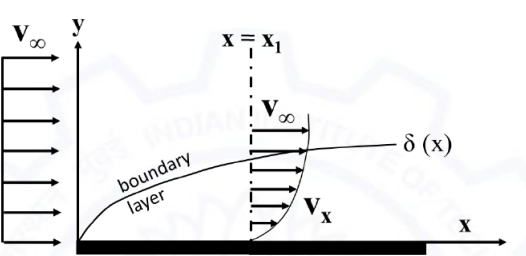
\includegraphics[width=0.4\columnwidth]{figs/Q.24.png}
    \caption\centering{PLATE OF FINITE LENGTH}
    \label{fig:placeholder}
\end{figure}


\item The vacancy concentration in a crystal doubles upon increasing the temperature from $27\degree$C to $127\degree$C. The enthalpy (in $kJ mol^{-1}$) of vacancy formation is: \underline {\hspace{2cm}} (round off to 2 decimal places). \\ Given: R = 8.314 J $mol^{-1} K^{-1}$ \hfill{\brak{\text{GATE MT 2021}}}
\end{enumerate}

\subsection*{Q36 - Q65 Multipe choice question carry two marks each  (for each wrong answer: - 2/3)}
\begin{enumerate}[resume]
\item The minimum value of y for the equation $y = x^2 - 2x + 4$ is \hfill{\brak{\text{GATE MT 2021}}}
\begin{multicols}{4}
\begin{enumerate}
\item 3
\item 1
\item 4
\item 6
\end{enumerate}
\end{multicols}

\item Match the forming process (in Column I) with its name (in Column II): \hfill{\brak{\text{GATE MT 2021}}}
\begin{figure}[H]
    \centering
    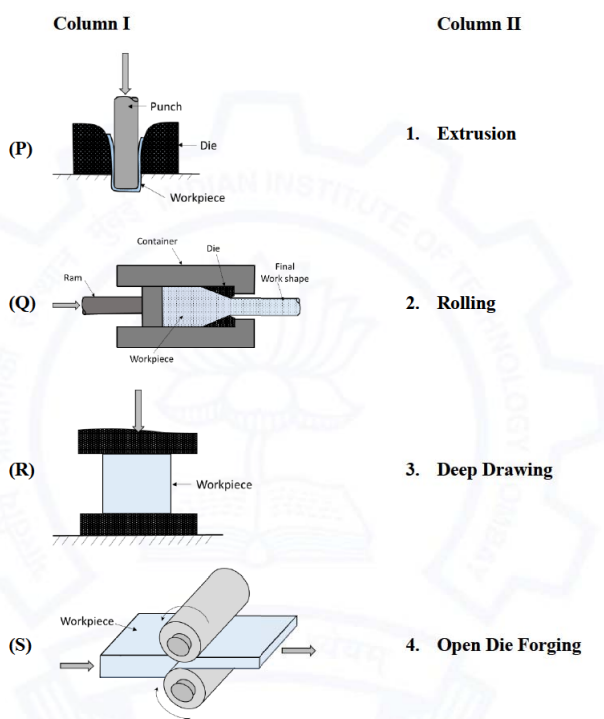
\includegraphics[width=0.8\columnwidth]{figs/Q.27.png}
    \caption\centering{FIGURE}
    \label{fig:placeholder}
\end{figure}
\begin{multicols}{2}
\begin{enumerate}
\item $P-1, Q-2, R-3, S-4$
\item $P-3, Q-1, R-4, S-2$
\item $P-3, Q-4, R-1, S-2$
\item $P-1, Q-4, R-3, S-2$
\end{enumerate}
\end{multicols}

\item Match the nondestructive technique (in Column I) with its underlying phenomenon (in Column II): \hfill{\brak{\text{GATE MT 2021}}}
\begin{center}
\begin{tabular}{ll}
\textbf{Column I} & \textbf{Column II} \\
(P) Dye penetrant test & 1. X-ray absorption \\
(Q) Radiography & 2. Capillary action \\
(R) Eddy current test & 3. Elastic waves reflection \\
(S) Ultrasonic inspection & 4. Electromagnetic induction \\
\end{tabular}
\end{center}
\begin{multicols}{2}
\begin{enumerate}
\item $P-4, Q-3, R-2, S-1$
\item $P-2, Q-1, R-3, S-4$
\item $P-2, Q-1, R-4, S-3$
\item $P-3, Q-2, R-1, S-4$
\end{enumerate}
\end{multicols}

\item Number of degrees of freedom for the following reacting system is: \hfill{\brak{\text{GATE MT 2021}}} 
\begin{align}
  M(s) + CO_2(g) = MO(s) + CO(g)
\end{align}

\begin{multicols}{4}
\begin{enumerate}
\item 0
\item 1
\item 2
\item 3
\end{enumerate}
\end{multicols}

\item The condition for getting the binary phase diagram of A-B (shown below) is: \hfill{\brak{\text{GATE MT 2021}}}
\begin{figure}[H]
    \centering
    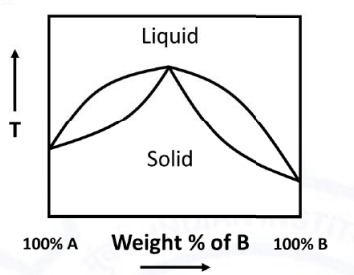
\includegraphics[width=0.3\columnwidth]{figs/Q.30.png}
    \caption\centering{BINARY PHASE DIAGRAM}
    \label{fig:placeholder}
\end{figure}
Given: $\Delta H_{mix}^{solid}$ - Enthalpy of mixing of solid \\ $\Delta H_{mix}^{liquid}$ - Enthalpy of mixing of liquid
\begin{multicols}{2}
\begin{enumerate}
\item $\Delta H_{mix}^{solid} = 0$ and $\Delta H_{mix}^{liquid} = 0$
\item $\Delta H_{mix}^{solid} < 0$ and $\Delta H_{mix}^{liquid} = 0$
\item $\Delta H_{mix}^{solid} > 0$ and $\Delta H_{mix}^{liquid} = 0$
\item $\Delta H_{mix}^{solid} = 0$ and $\Delta H_{mix}^{liquid} << 0$
\end{enumerate}
\end{multicols}

\item In the absence of any external stress, which one of the following statements related to the interaction of point defect and a dislocation is FALSE: \hfill{\brak{\text{GATE MT 2021}}}
\begin{enumerate}
\item An oversized solute atom would preferentially migrate below the slip plane of an edge dislocation
\item A spherically symmetric point defect can interact with both the hydrostatic and shear stress fields of a dislocation.
\item A point defect can locally modify the elastic modulus and thereby can change the interaction energy
\item Vacancies are attracted towards the compressive region of dislocation.
\end{enumerate}

\item A single crystal aluminium sample is subjected to uniaxial tension along
[112] direction. If the applied tensile stress is 100 MPa and the critical
resolved shear stress (CRSS) is 25 MPa, which one of the following slip
systems will be activated?

\hfill{\brak{\text{GATE MT 2021}}}
\begin{multicols}{4}
\begin{enumerate}
    \item $[101](111)$
    \item $[110](111)$
    \item $[101](111)$
    \item $[011](111)$
\end{enumerate}
\end{multicols}
\item One-dimensional steady-state temperature distribution in two adjacent
refractory blocks (with thermal conductivities, k1 and k2) of unit cross-
sectional area are shown below. The temperature T1 and thermal contact
resistance of the interface, respectively, are:\hfill{\brak{\text{GATE MT 2021}}}
\begin{figure}[H]
    \centering
    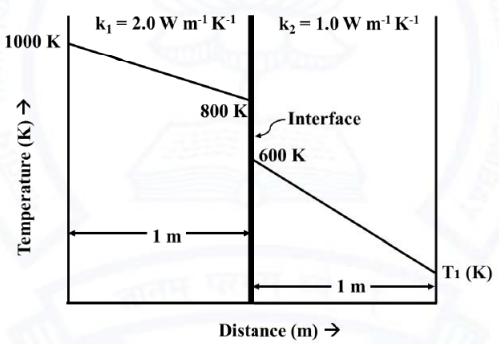
\includegraphics[width=0.5\columnwidth]{figs/Q.33.png}
    \caption\centering{ADJACENT REFRACTORY BLOCKS}
    \label{fig:placeholder}
\end{figure}
\begin{multicols}{2}
\begin{enumerate}
\item $200 K, 0.5 K W^{-1}$
\item $400 K, 1 K W^{-1}$
\item $200 K, 0.25 K W^{-1}$
\item $500 K, 0.5 K W^{-1}$
\end{enumerate}
\end{multicols}

\item For a fully developed 1-D flow of a Newtonian fluid through a horizontal
pipe of radius R (see figure), the axial velocity $(V_z)$ is given by: 
\begin{align}
    V_z=[\frac{\Delta P}{L}](\frac{R^2-r^2}{4\mu}),
\end{align}
where,$\Delta P$ is the pressure difference $(P1-P2)$, $\mu$ is the viscosity, $r$ is the radial distance from the axis and L is the length of the tube. The shear
stress exerted by the fluid on the tube wall is:
\begin{figure}[H]
    \centering
    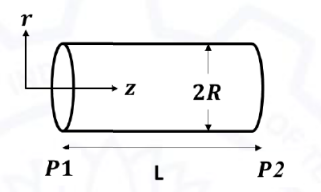
\includegraphics[width=0.5\columnwidth]{figs/Q.34.png}
    \caption\centering{HORIZONTAL PIPE}
    \label{fig:placeholder}
\end{figure}
 \hfill{\brak{\text{GATE MT 2021}}}
 \begin{multicols}{4}
\begin{enumerate}
\item $\frac{\Delta PR}{2L}$
\item $\frac{\Delta PR}{L}$
\item $\frac{3\Delta PR}{2L}$
\item $\frac{2\Delta PR}{L}$
\end{enumerate}
\end{multicols}

\item Match the terms (in Column I) with the unit process (in Column II)
\hfill{\brak{\text{GATE MT 2021}}}
\begin{center}
    

\begin{tabular}{ll}
 \textbf{Column I }    & \textbf{in Column II} \\
   (P) Submerged Entry Nozzle  & 1. Ladle Furnace\\
   (Q) Electric Heating& 2. Continuous Casting\\
   (R) Raceway Zone&3. LD Converter\\
   (S) Oxygen Lancing &4. Blast Furnace\\
\end{tabular}
\end{center}

\begin{multicols}{2}
\begin{enumerate}
\item $P-2,Q-1,R-4,S-3$
\item $P-4,Q-1,R-2,S-3$
\item $P-4,Q-3,R-1,S-2$
\item $P-2,Q-3,R-4,S-1$
\end{enumerate}
\end{multicols}
\item A blast furnace uses hematite ore with $80\% \;Fe_2O_3$ and $20\%$ gangue
materials. It uses 600 kg coke per ton of hot metal. The coke contains $85\%$
C and $15\%$ ash. The composition of hot metal is $95.5\%$ Fe and $4.5\% C$.
The weight of iron ore used and slag produced per ton of hot metal
respectively, are:\\
Assume that the gangue materials of the ore and ash content of coke form
slag while Fe2O3 in the ore is consumed in making hot metal.
\hfill{\brak{\text{GATE MT 2021}}}
\begin{multicols}{2}
\begin{enumerate}
\item $1705 kg, 431 kg$
\item $2131 kg, 546 kg$
\item $1705 kg, 331 kg$
\item $1500 kg, 431 kg$
\end{enumerate}
\end{multicols}
\subsection*{Q.37-Q.55 Numerical Answer Type (NAT), carry TWO mark each (no negative marks).}


\item Consider the function $f(x)=x-\cos{x}$. Using Newton-Raphson method,
the estimated root of $f(x)$ after the first iteration is:  \underline {\hspace{2cm}}. (round off to 3 decimal places).\\ 
Assume: Initial guess of the root = 0.5 radians
\hfill{\brak{\text{GATE MT 2021}}}

\item The work done by a force $\vec{F}=2xi
+3yj$  along a straight line from point $(0, 0)\; \text{to}\; (1, 2)$ is: \underline {\hspace{2cm}}. (round off to nearest integer). \hfill{\brak{\text{GATE MT 2021}}}

\item A coin is tossed three times. Given that there are more heads than tails, the
probability of getting exactly one tail is: \underline {\hspace{2cm}}. (round off to 2 decimal places). \hfill{\brak{\text{GATE MT 2021}}}

\item A continuous fillet weld is made using a $3000 W$ welding machine. At a
travel speed of $6 \;mm s^{-1}$, the cross-sectional area $(in\; mm^2)$ of the weld is: \underline {\hspace{2cm}}. (round off to nearest integer).\\
Given: The unit energy required to melt the metal is $6\; J mm^{-3}$.\\
Heat transfer factor = 0.6\\
Melting factor = 0.5
\hfill{\brak{\text{GATE MT 2021}}}

\item Liquid iron is cast into a spherical sand mold (6 cm radius) and a cubical
sand mold (12 cm edge length). If solidification time is 60 minutes in the
spherical casting, the time (in minutes) required to solidify in the cubical
casting is:  \underline {\hspace{2cm}}. (round off to nearest integer).  \hfill{\brak{\text{GATE MT 2021}}}

\item True strain for $60\%$ height reduction of a sample subjected to hot forging
is:\underline {\hspace{2cm}}. (round off to 2 decimal places). \hfill{\brak{\text{GATE MT 2021}}}

\item For the equilibrium reaction: $2Cu{(s)}+SO_2{(g)} = Cu_2S{(s)} +O_2{(g)}$, the
value of $\ln{\frac{P_{O_2}}{P_{SO_2}}}$ at 973 K is  \underline {\hspace{2cm}}. (round off to 2 decimal places).\\
Given: $2Cu{(s)}+0.5SO_2{(g)} = Cu_2S{(s)} $ $\Delta G\degree$ at 973 K = $-100 kJ$\\
$SO_2{(g)} = 0.5S_2 +O_2{(g)}$ $\Delta G\degree $ at 973 K = $292 kJ$\\
R = $8.314 J mol^{-1} K^{-1}$\\
Assume: Cu and $Cu_2S$ are pure solids.
\hfill{\brak{\text{GATE MT 2021}}}

\item One mole of an ideal gas at 10 atm. and 300 K undergoes reversible
adiabatic expansion to a pressure of one atm. The work done (in Joule) by
the gas is: \underline {\hspace{2cm}}. (round off to nearest integer). \hfill{\brak{\text{GATE MT 2021}}}

\item The figure shows the entropy versus temperature (S-T) plot of a reversible
cycle of an engine. If $T_1 = 200 K$ and $T_2 = 600 K$, the efficiency of the engine
(in percent) is:  \underline {\hspace{2cm}}. (round off to nearest integer). \hfill{\brak{\text{GATE MT 2021}}}
\begin{figure}[H]
    \centering
    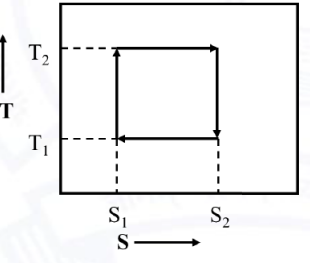
\includegraphics[width=0.5\columnwidth]{figs/Q.45.png}
    \caption\centering{ENTROPY VERSUS TEMPERATURE PLOT}
    \label{fig:placeholder}
\end{figure}

\item Two dislocation lines parallel to $z-axis$ lying in the $x-z$ plane are shown in
the figure. The glide force (in Newton) exerted by the edge dislocation on
the screw dislocation is:  \underline {\hspace{2cm}}.
\begin{figure}[H]
    \centering
    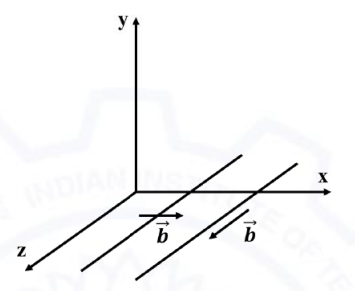
\includegraphics[width=0.5\columnwidth]{figs/Q.46.png}
    \caption\centering{3D PLANE}
    \label{fig:placeholder}
\end{figure}
For the edge, the shear stress component is given by:
\begin{align}
    \tau_{xy}=\frac{Gb}{2\pi(1-v)}\frac{x(x^2-y^2)}{(x^2+y^2)^2}
\end{align}
Given: Shear modulus, $G = 28 GPa$\\
Poisson's ratio, $\nu = 0.3$\\
Burgers vector, $b = 0.29 nm$\\
Distance between the two dislocations = 0.5 nm

\item In a material, a shear stress of $100 MPa$ is required to bow a dislocation
line between precipitates with a spacing of $0.2 \micro m$. If the spacing between
the precipitates is increased to $0.5 \micro m$, the shear stress (in MPa) to bow the
dislocation would be: \underline {\hspace{2cm}}. (round off to nearest integer ). \hfill{\brak{\text{GATE MT 2021}}}

\item A metal plate is in a state of plane strain $(\epsilon_{zz}=0)$ with $\sigma_{xx}=\sigma_{yy}\neq0$  and $\tau_{xy}=\tau_{xz}=\tau_{yz}$ If the Poisson's ratio is 0.3, the ratio, $\sigma_{zz} / \sigma_{xx}$\underline {\hspace{2cm}}. (round off to 1 decimal places). \hfill{\brak{\text{GATE MT 2021}}}

\item An infinite metal plate has a central through-thickness crack of length $\frac{80}{\pi}$ mm. The maximum applied stress (in MPa) that the plate can sustain in
mode I is:  \underline {\hspace{2cm}}. (round off to nearest integer).\\
Assume: Linear elastic fracture mechanics is valid\\
Given: Fracture toughness,$K_{IC}=20MPa\;m^{1/2}$
\hfill{\brak{\text{GATE MT 2021}}}

\item A hypothetical binary eutectic phase diagram of A-B is shown below. An
alloy with $5 wt.\%$ B solidifies with no convection. Assuming steady state,
the critical temperature gradient $(in\; K \;mm^{-1})$ required to maintain planar
solidification front is:  \underline {\hspace{2cm}}. (round off to nearest integer). \hfill{\brak{\text{GATE MT 2021}}}
\begin{figure}[H]
    \centering
    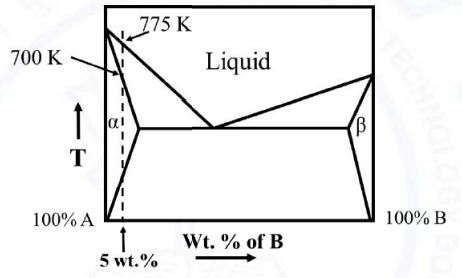
\includegraphics[width=0.5\linewidth]{figs/Q.50.png}
    \caption\centering{PHASE DIAGRAM}
    \label{fig:placeholder}
\end{figure}
Given: Diffusivity of B in liquid = $10^{-9} m^2 s^{-1}$\\
Velocity of solidification front = $4\; \micro m \;s^{-1}$

\item A thick steel plate containing $0.1 wt.\% C$ is carburized at $950\degree C$. The
plate's surface carbon concentration is maintained at $1.1 wt.\% C$. After 9
hours, the depth (in mm) below the surface at which the carbon
concentration is $0.6 wt.\% C$ will be:  \underline {\hspace{2cm}}. (round off to 2 decimal places). \hfill{\brak{\text{GATE MT 2021}}}\\
Given: Diffusivity of carbon in $\gamma-Fe$ at $950\degree C = 1.6\times10^{-11} m^2 s^{-1}$\\
Error function table:\\
\begin{tabular}{lllllll}
  z &0.35&0.40&0.45&0.50&0.55&0.60  \\
   erf(z)  &0.3794&0.4284&0.4755&0.5205&0.5633&0.6039 
\end{tabular}

\item At $25\degree C$, iron corrodes in a deaerated acid of pH 3 with a corrosion
current density of $4 \micro A\;cm^{-2}$. The corrosion potential (V) is:  \underline {\hspace{2cm}}. (round off to 2 decimal places). \hfill{\brak{\text{GATE MT 2021}}}\\
Given: $\beta_c = 0.1 V$ per decade of current density\\
Exchange current density of hydrogen on iron surface = $10^{-9}\; A\; cm^{-2}$\\
R = $8.314 J mol^{-1} K^{-1}, F = 96500 C mol^{-1}$\\
All potentials are with reference to standard hydrogen electrode.

\item The radius of an interstitial atom which just fits (without distorting the
structure) inside an octahedral void of a bcc-iron crystal (in nm) is: \underline {\hspace{2cm}}  (round off to 3 decimal places). \\ Assume the radius of Fe atom to be $0.124 nm$ \hfill{\brak{\text{GATE MT 2021}}}

\item Nickel undergoes isothermal oxidation at $800 K$ for a duration of $400 s$
resulting in a weight gain of $2 \;mg \;cm^{-2}$. The weight gain $(mg\; cm^{-2})$ after a duration of 1600 s is:  \underline {\hspace{2cm}}. (round off to nearest integer). \hfill{\brak{\text{GATE MT 2021}}}\\
Assume: Weight gain is proportional to square root of time

\item A solid sphere (0.5 m radius) is enclosed within a larger hollow sphere (1 m
radius), as shown in figure. The radiation exchange takes place between the
outer surface (surface 1) of the small sphere and the inner surface (surface
2) of the bigger sphere. The value of the view factor, $F_{22}$ is:  \underline {\hspace{2cm}}. (round off to 2 decimal places). \hfill{\brak{\text{GATE MT 2021}}}\\
Given: View factor $(F_{ij})$ is the fraction of the radiation leaving surface i
that is intercepted by surface j.
\begin{figure}[H]
    \centering
    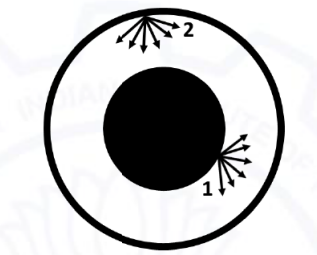
\includegraphics[width=0.5\columnwidth]{figs/Q.55.png}
    \caption\centering{SOLID SPHERE}
    \label{fig:placeholder}
\end{figure}

\end{enumerate}
\section*{*END OF THE QUESTION PAPER*}
 
\end{document}